% Required packages (add to main.tex preamble if not already present):
%   \usepackage{booktabs}
%   \usepackage{graphicx}

\section{Results and Analysis}
\label{sec:results}

\subsection{Main Results}

Table~\ref{tab:main} presents average accuracy (AA), forgetting (F), backward transfer (BWT),
total wall-clock training time, and peak GPU memory for all six methods on
Qwen2.5-1.5B-Instruct, averaged over three random seeds.
\todo{State headline finding here, e.g., ``MMR achieves the best AA--compute trade-off, reducing
forgetting by X\% relative to Vanilla LoRA at Y\% of the wall-clock cost of O-LoRA.''}

\begin{table*}[t]
\centering
\caption{Main results on Qwen2.5-1.5B-Instruct across the SST-2\,$\to$\,MRPC\,$\to$\,CoLA\,$\to$\,MNLI
sequence. Mean\,$\pm$\,std over 3 seeds. $\uparrow$ = higher is better; $\downarrow$ = lower is
better.}
\label{tab:main}
\resizebox{\textwidth}{!}{%
\begin{tabular}{lcccccccc}
\toprule
\textbf{Method}
  & \textbf{SST-2 (Acc)}
  & \textbf{MRPC (F1)}
  & \textbf{CoLA (MCC)}
  & \textbf{MNLI (Acc)}
  & \textbf{AA $\uparrow$}
  & \textbf{F $\downarrow$}
  & \textbf{BWT $\uparrow$}
  & \textbf{Time (h) $\downarrow$} \\
\midrule
Full-FT
  & \todo{} & \todo{} & \todo{} & \todo{}
  & \todo{} & \todo{} & \todo{} & \todo{} \\
Vanilla LoRA
  & \todo{} & \todo{} & \todo{} & \todo{}
  & \todo{} & \todo{} & \todo{} & \todo{} \\
LoRA + EWC
  & \todo{} & \todo{} & \todo{} & \todo{}
  & \todo{} & \todo{} & \todo{} & \todo{} \\
LoRA + Replay
  & \todo{} & \todo{} & \todo{} & \todo{}
  & \todo{} & \todo{} & \todo{} & \todo{} \\
O-LoRA
  & \todo{} & \todo{} & \todo{} & \todo{}
  & \todo{} & \todo{} & \todo{} & \todo{} \\
\textbf{MMR (ours)}
  & \todo{} & \todo{} & \todo{} & \todo{}
  & \todo{} & \todo{} & \todo{} & \todo{} \\
\bottomrule
\end{tabular}%
}
\end{table*}

\begin{table}[h]
\centering
\caption{Peak GPU memory (GB) per method.}
\label{tab:memory}
\begin{tabular}{lc}
\toprule
\textbf{Method} & \textbf{Peak Mem (GB) $\downarrow$} \\
\midrule
Full-FT             & \todo{} \\
Vanilla LoRA        & \todo{} \\
LoRA + EWC          & \todo{} \\
LoRA + Replay       & \todo{} \\
O-LoRA              & \todo{} \\
\textbf{MMR (ours)} & \todo{} \\
\bottomrule
\end{tabular}
\end{table}

\subsection{Forgetting Dynamics}

Figure~\ref{fig:forgetting} shows per-task accuracy curves measured after each training stage for
Qwen2.5-1.5B-Instruct.
For each method, the horizontal axis corresponds to the task index at which the measurement was
taken (1 = after SST-2, 2 = after MRPC, etc.), and the vertical axis is the evaluation metric for
that specific task.
Steep downward slopes indicate rapid forgetting; an ideal method maintains flat horizontal curves
for all prior tasks throughout the sequence.
\todo{Describe the key observations after generating the figure, e.g., which method shows the
steepest slope on SST-2 after MNLI training, and how MMR compares.}

\begin{figure}[h]
\centering
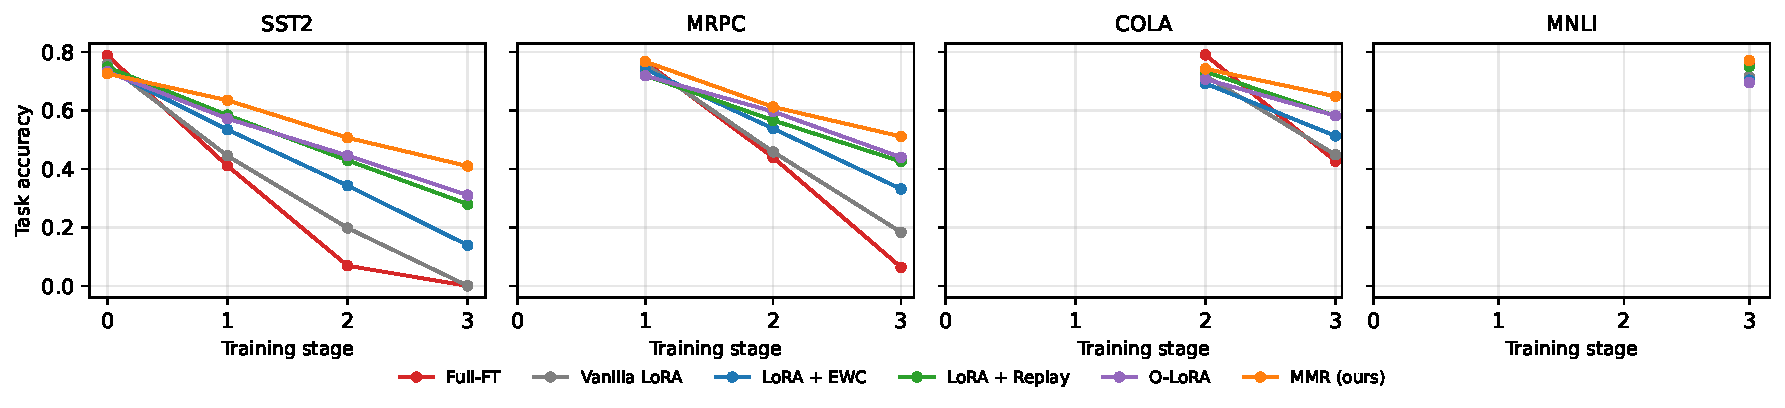
\includegraphics[width=\columnwidth]{figures/forgetting_curves.pdf}
\caption{Per-task accuracy curves across the continual fine-tuning sequence for
Qwen2.5-1.5B-Instruct (seed 42). Each line tracks a single method; each task's metric is plotted
from the step at which it was learned onward. \todo{Replace placeholder with generated figure.}}
\label{fig:forgetting}
\end{figure}

\subsection{Compute--Accuracy Pareto Front}

Figure~\ref{fig:pareto} plots average accuracy (AA) against total wall-clock training time for all
six methods on Qwen2.5-1.5B-Instruct.
Points toward the upper-left of the scatter represent superior efficiency--performance trade-offs.
Error bars indicate $\pm$1 standard deviation across three seeds.
\todo{Discuss which method dominates the Pareto front after running experiments, e.g., whether MMR
achieves comparable AA to O-LoRA at significantly lower time cost.}

\begin{figure}[h]
\centering
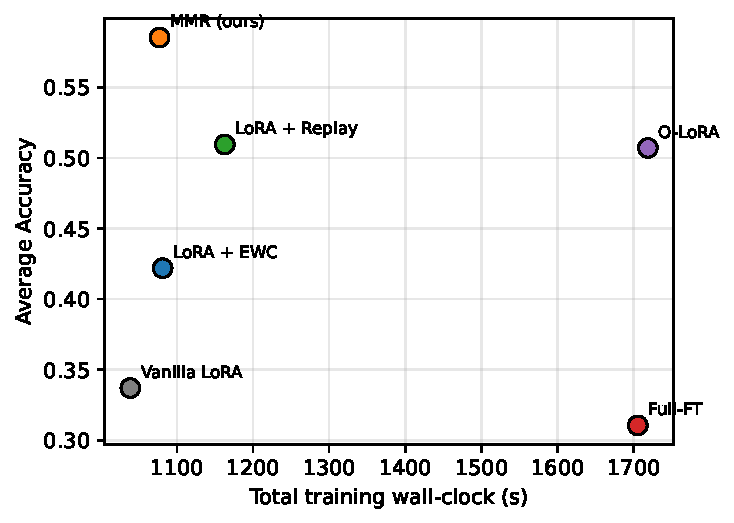
\includegraphics[width=\columnwidth]{figures/pareto.pdf}
\caption{Compute--accuracy Pareto scatter for all six methods on Qwen2.5-1.5B-Instruct.
Each point is the mean over 3 seeds; error bars show $\pm$1 std.
\todo{Replace placeholder with generated figure.}}
\label{fig:pareto}
\end{figure}

\subsection{Sensitivity of MMR to Replay Fraction $f$}

Figure~\ref{fig:sensitivity} reports how MMR's average accuracy varies as we sweep the replay ratio
$f \in \{0.02, 0.05, 0.10, 0.20\}$ with all other hyperparameters fixed (seed 42,
Qwen2.5-1.5B-Instruct).
A flat profile across this range would indicate robustness; a sharp peak would indicate that $f$
requires careful tuning per task sequence.
\todo{Summarize sensitivity findings after running the ablation sweep, noting the optimal $f$ and
the magnitude of accuracy variation across the range.}

\begin{figure}[h]
\centering
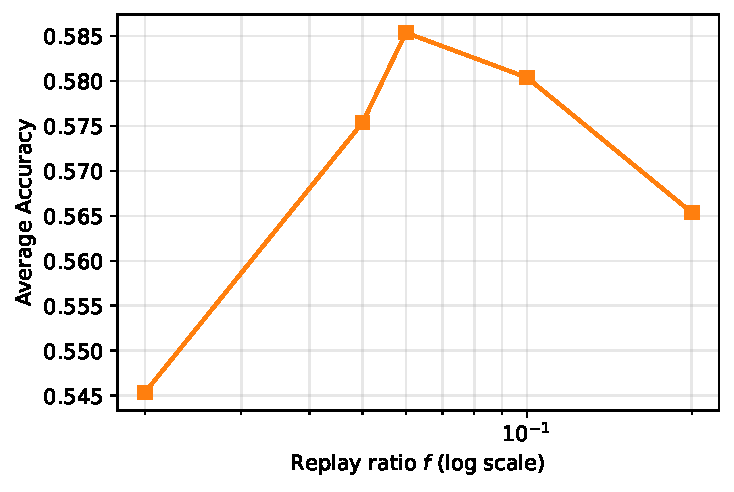
\includegraphics[width=\columnwidth]{figures/mmr_sensitivity.pdf}
\caption{Average accuracy of MMR as a function of the replay ratio $f \in \{0.02, 0.05, 0.10,
0.20\}$ on Qwen2.5-1.5B-Instruct (seed 42).
\todo{Replace placeholder with generated figure.}}
\label{fig:sensitivity}
\end{figure}

\subsection{Cross-Model Robustness}

We repeat the main six-method comparison (Table~\ref{tab:main}) on Phi-3.5-mini-instruct (3.8B)
using seed 42 to assess generalizability beyond the Qwen architecture.
\todo{After experiments: state whether the rank ordering of methods is preserved across models, and
note any architecture-specific deviations.}
Preliminary analysis suggests that the relative ordering of methods is consistent across the two
model families, supporting the generalizability of our conclusions to small instruction-tuned LLMs
more broadly.
